\documentclass[12pt]{article}

\usepackage{graphicx}
\usepackage{amsmath}
\usepackage{amssymb}
\usepackage{natbib}
\usepackage{amsfonts}
\usepackage{multicol}
\usepackage{float}
\usepackage{oldgerm}
\usepackage{bm}
\usepackage{mathtools}
\usepackage{wrapfig}
\usepackage{fancyhdr}
\usepackage[export]{adjustbox}
\usepackage{xcolor}

\pagestyle{empty}

\newcommand{\Avec}{\mathbf A}
\newcommand{\Bvec}{\mathbf B}
\newcommand{\Dvec}{\mathbf D}
\newcommand{\Evec}{\mathbf E}
\newcommand{\Fvec}{\mathbf F}
\newcommand{\Jvec}{\mathbf J}
\newcommand{\Lvec}{\mathbf L}
\newcommand{\Mvec}{\mathbf M}
\newcommand{\Pvec}{\mathbf P}
\newcommand{\Svec}{\mathbf S}
\newcommand{\avec}{\mathbf a}
\newcommand{\bvec}{\mathbf b}
\newcommand{\dvec}{\mathbf d}
\newcommand{\evec}{\mathbf e}
\newcommand{\fvec}{\mathbf f}
\newcommand{\jvec}{\mathbf j}
\newcommand{\kvec}{\mathbf k}
\newcommand{\nvec}{\mathbf n}
\newcommand{\pvec}{\mathbf p}
\newcommand{\rvec}{\mathbf r}
\newcommand{\svec}{\mathbf s}
\newcommand{\vvec}{\mathbf v}
\newcommand{\xvec}{\mathbf x}
\newcommand{\yvec}{\mathbf y}
\newcommand{\zvec}{\mathbf z}
\newcommand{\nablav}{\boldsymbol{\nabla}}
\newcommand{\nablavector}{\vec \nabla}
\newcommand{\alphavec}{\boldsymbol{\alpha}}
\newcommand{\phivec}{\boldsymbol{\phi}}
\newcommand{\thetavec}{\boldsymbol{\theta}}
\newcommand{\omegavec}{\boldsymbol{\omega}}
\newcommand{\tauvec}{\boldsymbol{\tau}}
\newcommand{\ezero}{\varepsilon_{0}}
\newcommand{\mzero}{\mu_{0}}
\newcommand{\mubold}{\boldsymbol{\mu}}
\newcommand{\uniti}{\hat{\boldsymbol{\imath}}}
\newcommand{\unitj}{\hat{\boldsymbol{\jmath}}}
\newcommand{\unitk}{\hat{\boldsymbol{\mathit{k}}}}
\newcommand{\unitn}{\hat{\mathbf n}}
\newcommand{\unitr}{\hat{\mathbf r}}
\newcommand{\unitphi}{\hat{\boldsymbol{\phi}}}
\newcommand{\unittheta}{\hat{\boldsymbol{\theta}}}

\newcommand{\bit}{\begin{itemize}}
\newcommand{\eit}{\end{itemize}}

\setlength{\headsep}{0.5cm}
\setlength{\oddsidemargin}{-0.5cm}
\setlength{\textwidth}{16.5cm}
\setlength{\textheight}{24cm}
\voffset = -2cm

\pagestyle{fancy}
\fancyhf{}
\rfoot{
\includegraphics[width=1.0in]{cnm.png}}
\lfoot{ENGR 2910 Homework 5}
\begin{document}

%{\bf \underline{STUDENT NAME}:} 
%\vspace{1cm}

\begin{center}
%\date{10/02/18-10/09/18}
\hfil
{\large\bf {ENGR 2910-101: Circuit Analysis}}
\hfill Instructor: Leo Silbert \\
Homework 5: 09/28/21 \hfill Due: 10/05/21\\
\hrulefill\\
\end{center}

%{\em Show all your working to ensure you obtain full points. Partial
%  credit will be given for correct algebraic steps if you fail to
%  obtain the correct final answer.}\\

%\newpage


\noindent
{\bf Question 1} [10] %P3-3

For each of the circuits (a)-(d), find the equivalent resistance and the power delivered by the source. 
\begin{figure}[h!]
  \centering 
 \vspace{-0.1in}
 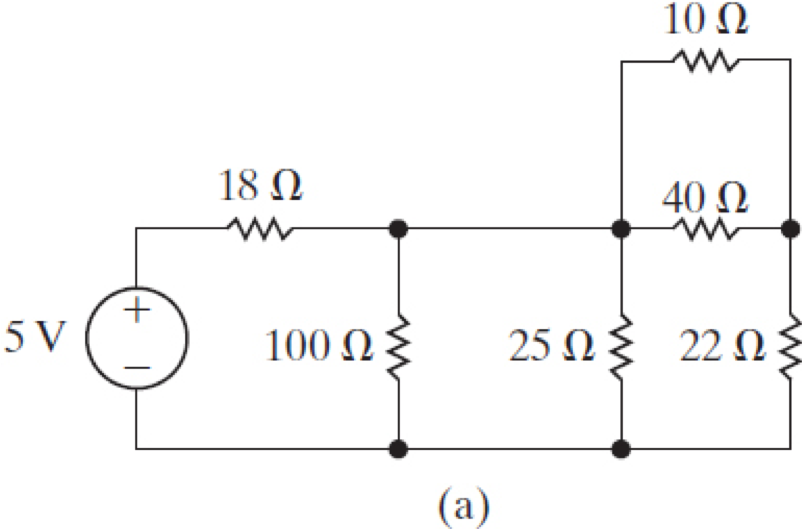
\includegraphics[clip,width=0.45\textwidth]{Fig3-3a.png}
 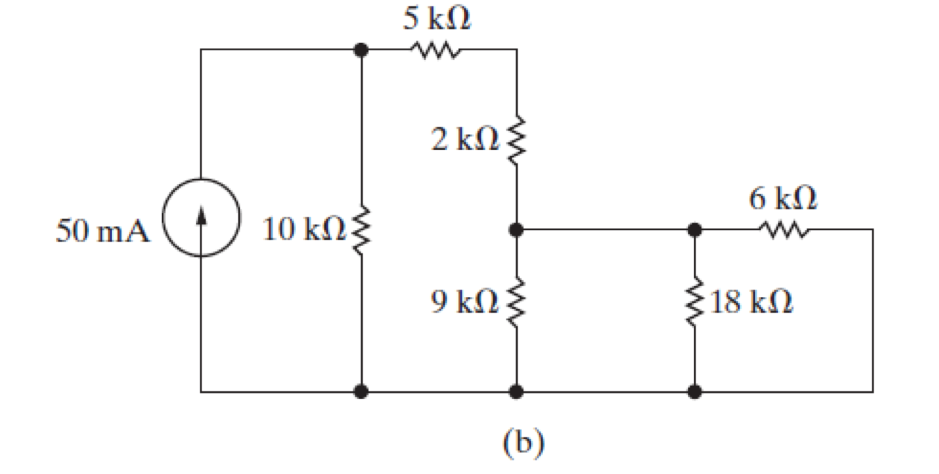
\includegraphics[clip,width=0.45\textwidth]{Fig3-3b.png}\\
 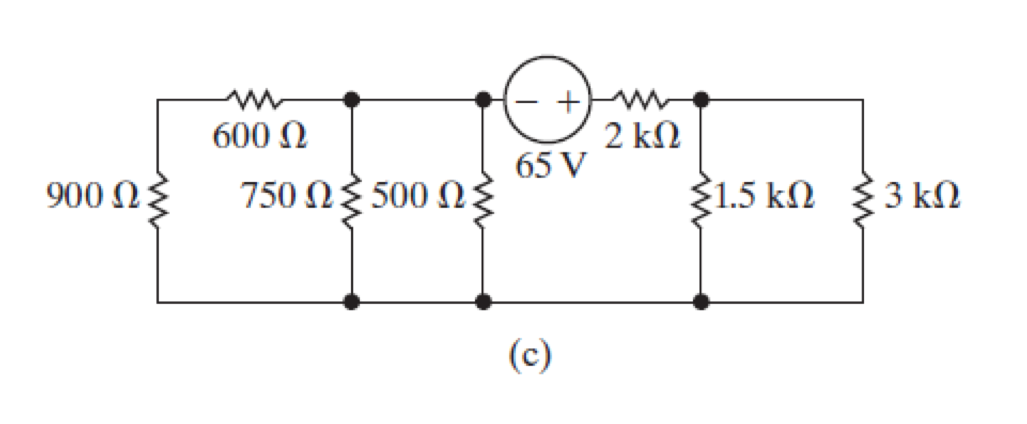
\includegraphics[clip,width=0.45\textwidth]{Fig3-3c.png}
 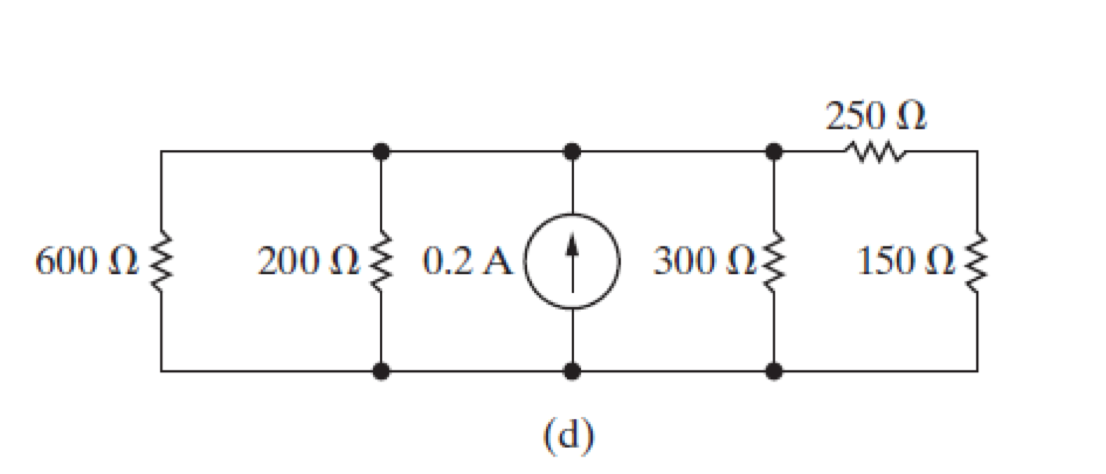
\includegraphics[clip,width=0.45\textwidth]{Fig3-3d.png}
%\vspace{-0.1in}
\end{figure}

\vspace{0.1in}
\noindent
{\bf Question 2} [10] %P3-5(d)

Find the equivalent resistance $R_{ab}$ for the following circuit.
\begin{figure}[h!]
     \centering
\vspace{-0.1in}
     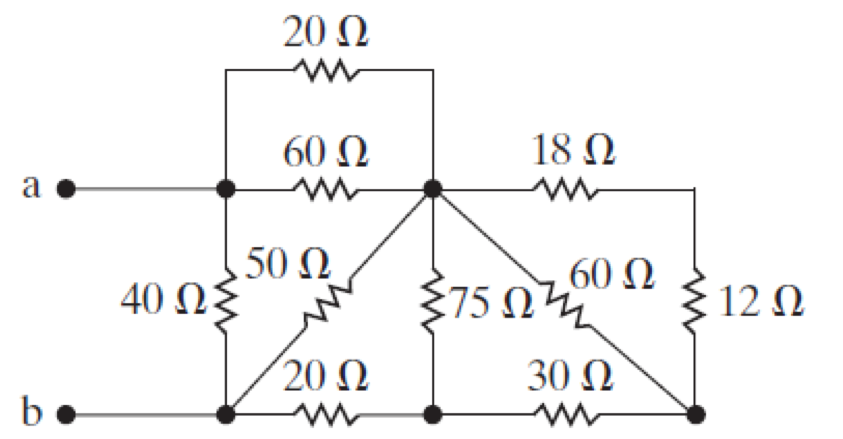
\includegraphics[clip,width=0.6\textwidth]{Fig3-6d.png}
\vspace{-0.15in}
\end{figure}
 \newpage
\noindent
{\bf Question 3} [10] %openstax

A battery of 45 V delivers 112 W of power to the circuit that contains 5 identical resistors (R$_{i}$=R). What is the value of R?

\begin{figure}[!h]
  \centering 
  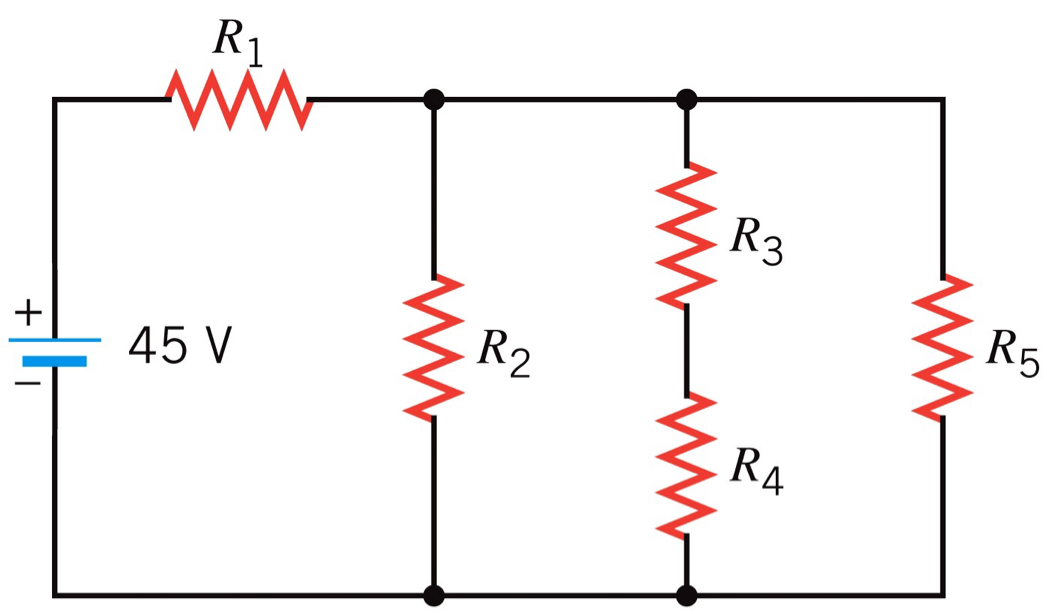
\includegraphics[clip,width=0.4\textwidth]{Fig-Q3.png}
\end{figure}

\vspace{0.1in}
\noindent
{\bf Question 4} [10] %P3-13

For the voltage-divider circuit shown: 
\begin{figure}[h!]
  \centering 
  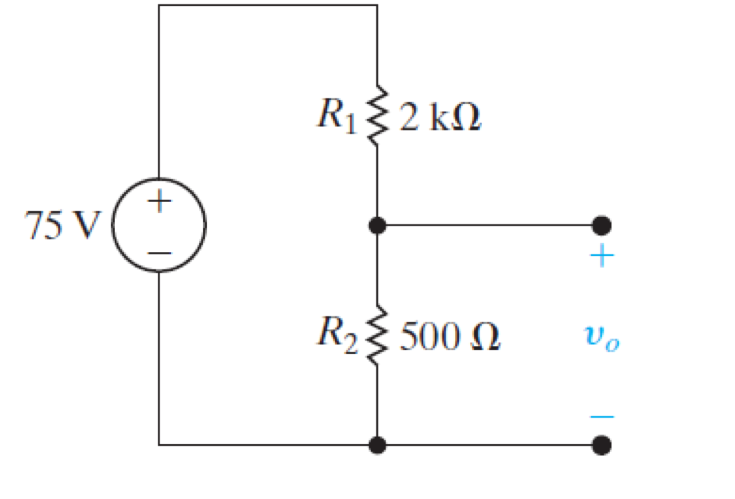
\includegraphics[clip,width=0.4\textwidth]{Fig3-13.png}
\end{figure}
\bit

\item[(a)]

Calculate the no-load voltage $v_{o}$.

\item[(b)]

Calculate the power dissipated in $R_{1}$ and $R_{2}$.

\item[(c)]

If only 1 W resistors are available and that the no-load voltage is to be the same as in part (a), specify the smallest values of $R_{1}$ and $R_{2}$.

\eit

\vspace{0.1in}
\noindent
{\bf Question 5} [10] %P3-1/2

For the circuit circuit shown:
\begin{figure}[h!]
\centering 
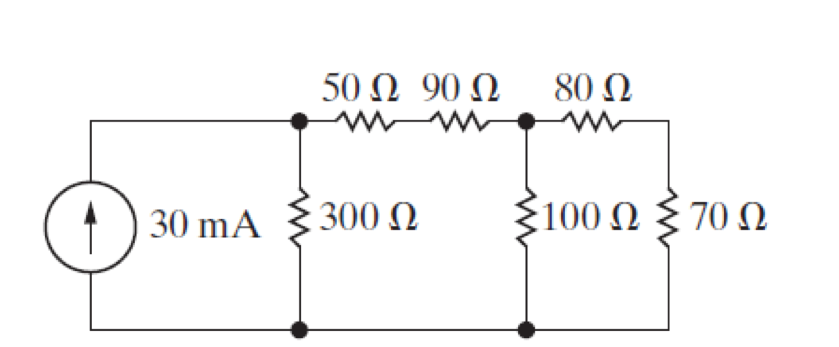
\includegraphics[clip,width=0.6\textwidth]{Fig3-1d.png}
\end{figure}
 
\bit

\item[(a)]

Use current division to find the current in the $50 \Omega$ resistor from left to right.

\item[(b)]

Use the result from part (a) and current division to find the current in the $70 \Omega$ resistor from top to bottom.

\eit

\end{document}
